% id: 0323
% book: RPM 중3-2 수학 · 03 원과 직선
% section: 유형 15 원에 외접하는 사각형의 성질 (1)
% figure: crop:fig-0323.png
% answer: ②
% answer_source: 답지
% variant_level: 0 (원본 전사)
% 이 파일은 build.mjs 가 items.json 에서 만든다. 고칠 때는 items.json 을 고친다.
\noindent\begin{minipage}[t]{0.58\linewidth}\vspace{0pt}\raggedright 오른쪽 그림에서 $\square\pt{ABCD}$는 원~$\pt{O}$에 외접하는 등변사다리꼴이고 $\seg{AD}=8\mkern3mu \mathrm{cm}$, $\seg{BC}=12\mkern3mu \mathrm{cm}$일 때, $\seg{AB}$의 길이는?\end{minipage}\hfill\begin{minipage}[t]{0.4\linewidth}\vspace{0pt}\centering \setlength{\dmfigw}{79.5pt}\ifdim\dmfigw>\linewidth\setlength{\dmfigw}{\linewidth}\fi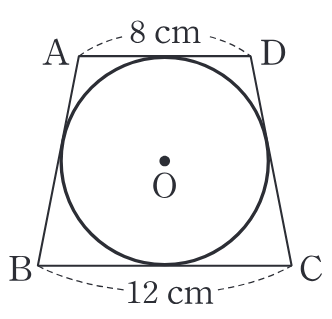
\includegraphics[width=\dmfigw]{figures/fig-0323.png}\end{minipage}\par
\begin{choicesii}{$8\mkern3mu \mathrm{cm}$}{$10\mkern3mu \mathrm{cm}$}{$12\mkern3mu \mathrm{cm}$}{$14\mkern3mu \mathrm{cm}$}{$16\mkern3mu \mathrm{cm}$}\end{choicesii}
